\section{Triangle Centers}
\label{app:Atri-ctrs}

Let $\mathbb{T}$ be the set of all triples $(a, b, c)$ of real numbers that are sidelengths of a triangle $ABC$. That is,
\[
\mathbb{T} = \{ (a, b, c): 0 <a< b + c, 0 <b < c +a, 0 < c < a+ b\}.\]

On any subset $U$ of $\mathbb{T}$, define a center  function as a nonzero function $f(a, b, c)$ such that:

\noindent i) $f$ is homogeneous in $a$, $b$, $c$ (i.e., $f(ta, tb, tc) = t^n f(a, b, c)$   for some non negative integer
$n$,  $t > 0$, and all $(a, b, c) $ in $U$.

\noindent ii) $f$ is  symmetric in $b$ and $c$ (i.e., $f(a, c, b)= f(a, b, c)$
for all $(a, b, c)$ in U. 


A center on $U$ is an equivalence class $[p,q,r]$ of ordered triples
$(p,q,r) $ given by
 \[p= f( a, b, c),\;\; q= f( b, c, a),\; r = f( c, a, b)\]
for some center function $f$ defined on $U$. 

\begin{remark}
 Also, it is useful to express the center functions in terms of the angles of the triangle using the relations of the triangle (law of cosines and sines).
\end{remark}
 
Trilinears coordinates $[p,q,r]$  of a point $X=(x,y) \in \mathbb{R}^2$ can be  converted to cartesians coordinates using \cite{mw}:

\begin{equation}
\label{eqn:appAtrilin-cartesian}
X=\frac{p a A + q b B + r c C}{pa+q b+r c}
\end{equation}
where $A=(x_a,y_a)$, $B=(x_b,y_b)$, $C=(x_c,y_c)$ are the vertices of the triangle $ABC$ expressed in cartesian coordinates.

The conversion of cartesians  to trilinears can be done as follows.

Consider a triangle $T=ABC$ with vertices $A=(x_a,y_a),$ $B=(x_b,y_b)$ and $C=(x_c,y_c)$.

Given a point $P=(x_0,y_0)$ the trilinear coordinates of $P$
is given by
{\small 
\[ \left[ \frac{1}{a}( (C-B)\wedge P+B\wedge C): \frac{1}{b}( (A-C)\wedge P+C\wedge A): \frac{1}{c}( (B-A)\wedge P+A\wedge B)\right] \]}
Here $u\wedge v$ is the area of the oriented parallelogram generated by $u$ and $v$.

\begin{remark}
In this book, also it will  frequently used the notation for a triangle: vertices $A=P_1$, $B=P_2$, $C=P_3$ and sidelengths $a=s_1=|P_2-P_3|$, $b=s_2=|P_1-P_3|$,
$c=s_3=|P_1-P_2|$.
\end{remark}

\begin{remark} \label{rem:baricentro_coord}
Another homogeneous coordinates are the so called {barycentrics}. If the   trilinear coordinates of a point is $[p,q,r]$  then its barycentric coordinates is $[ap,bq,cq]$. Observe that $2ap$ is the oriented area of the triangle $[AXB]$. Analogously, $2bq$ (resp. $2cr$) is the oriented area of the triangle $CXA$ (resp. $BXC$).
\end{remark}

\subsection*{Basic Constructions}

Constructions for a few basic Triangle Centers are shown in \cref{fig:constructions}.

\begin{figure}[H]
    \centering
   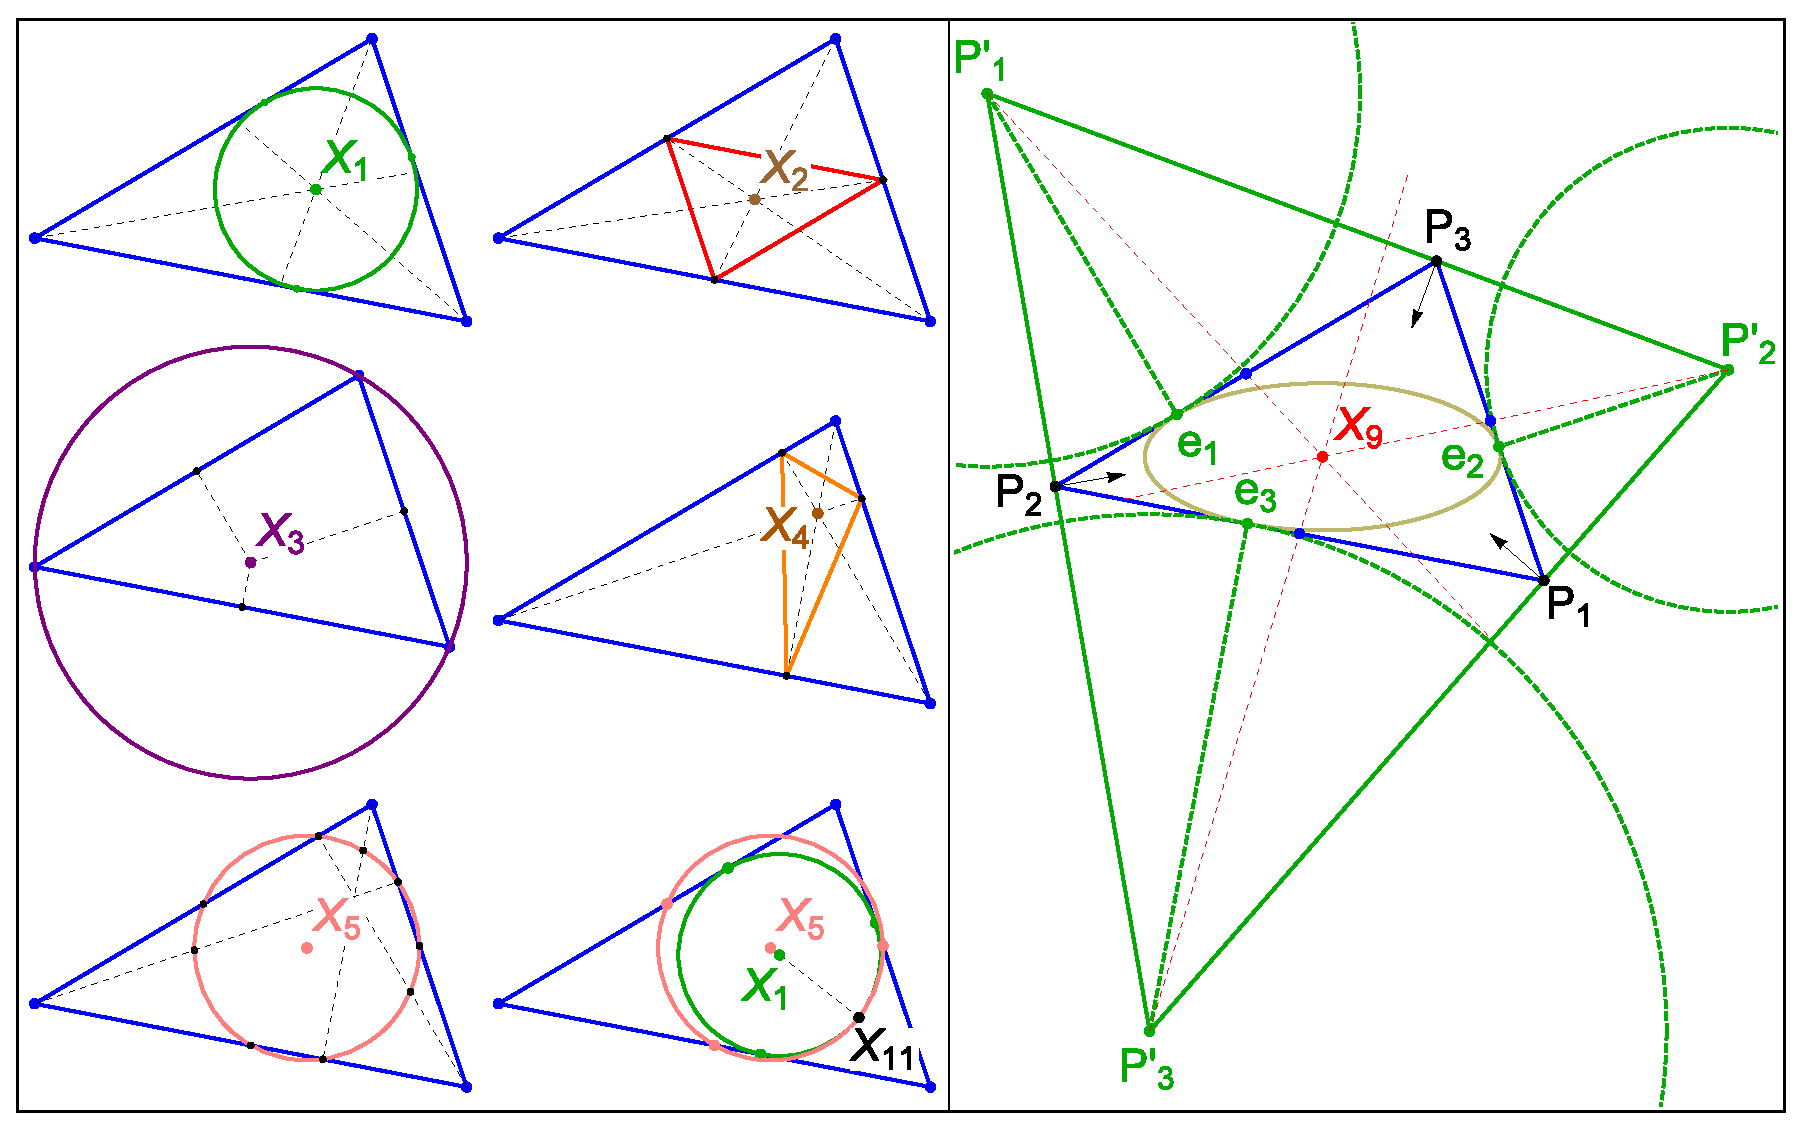
\includegraphics[width=\textwidth]{zappA/pics/pics_appA_010_constr.eps}
    \caption{Constructions for Triangle Centers $X_i$, $i=1,2,3,4,5,9,11$, taken from \cite{reznik2020-intelligencer}.}
    \label{fig:constructions}
\end{figure}

\begin{itemize}
    \item The incenter $X_1$ is the intersection of angular bisectors, and center of the incircle (green), a circle tangent to the sides at three {\em intouchpoints} (green dots), its radius is the {\em inradius} $r$.
    \item The barycenter $X_2$ is where lines drawn from the vertices to opposite sides' midpoints meet. Side midpoints define the {\em medial Triangle} (red).
    \item The circumcenter $X_3$ is the intersection of perpendicular bisectors, the center of the {\em circumcircle} (purple) whose radius is the {\em circumradius} $R$.
    \item The orthocenter $X_4$ is where altitudes concur. Their feet define the {\em orthic oriangle} (orange).
    \item $X_5$ is the center of the 9-Point (or Euler) circle (pink): it passes through each side's midpoint, altitude feet, and Euler Points \cite{mw}.
    \item The Feuerbach point $X_{11}$ is the single point of contact between the Incircle and the 9-Point circle.
    \item Given a reference triangle $P_1P_2P_3$ (blue), the {\em excenters} $P_1'P_2'P_3'$ are pairwise intersections of lines through the $P_i$ and perpendicular to the bisectors. This triad defines the {\em excentral triangle} (green).\
    \item The {\em excircles} (dashed green) are centered on the excenters and are touch each side at an {\em extouch point} $e_i,i=1,2,3$.
    \item Lines drawn from each excenter through sides' midpoints (dashed red) concur at the {\em Mittenpunkt} $X_9$.
    \item Also shown (brown) is the triangle's {\em Mandart inellipse}, internally tangent to each side at the $e_i$, and centered on $X_9$.
    %This is identical to the $N=3$ Caustic.
\end{itemize}

\begin{table}[H]
    \centering
    \begin{tabular}{|c|c|c|}
    \hline
         $X_k $& triangle center& $f(a,b,c)$ \\
         \hline
     $X_1 $ & incenter & $ 1$ \\
     \hline
          $X_2 $ & barycenter  & ${1}/{a}$ \\
          \hline
              $X_3$ & circumcenter & $\cos A$ \\
              \hline 
              $ X_4$ & orthocenter & $\sec A$ \\
              \hline   
                $X_5$ & center of Euler's circle & $\cos(B - C)$ \\
              \hline  
                $X_6$ & symmedian & $a$ \\
              \hline  
              $X_9$ & mittenpunkt & $b + c - a$ \\
              \hline
                 $X_{11}$ &Feuerbach point  & $1 - \cos(B - C)$ \\
              \hline
               $X_{15}$ & 1st isodynamic point   & $\sin(A+\frac{\pi}{3})$ \\
              \hline
                $ X_{16} $ & 2nd isodynamic point   & $\sin(A-\frac{\pi}{3})$ \\
              \hline
               $X_{33}$ &  \makecell[cc]{perspector of the orthic\\and intangents triangles}  & $1 +\sec{A}$ \\
            \hline
            %  $X_{88}$ & ss & $1/(b+c-2a)$ \\
         %     \hline
    \end{tabular}
    \caption{Some triangle centers and their first trilinear coordinate expressed as a symmetric function $f(a,b,c)$ on the sidelengths. The complete trilinear vector is given cyclically by $[f(a,b,c),f(b,c,a),f(c,a,b)]$. Note that sometimes these are more concisely expressed as trig functions on the angles $A,B,C$ which can be converted back to $f(a,b,c)$ via the law of sines and/or cosines.}
    \label{tab:Xitrilinear}
\end{table}

\begin{proposition}
The trilinear coordinates of $X_2$ are given by $[1/a,1/b,1/c].$
\end{proposition}

\begin{proof}
Consider a triangle of reference $T=ABC$. The midpoint of the segment $BC$ has trilinear coordinates $[0,1/b,1/c].$
In fact,
\begin{align*}
    [0,\frac{a}{2}\sin C, \frac{a}{2}\sin B] &\equiv[0,\sin C,\sin B]=[0,\sin C,\sin B]\\
    &\equiv[0,\frac{R}{b},\frac{R}{c}]\equiv [0,\frac{1}{b},\frac{1}{c}].
\end{align*} 
Analogously, $[1/a,0,1/c]$ and $[1/a,1/b,0]$ are the trilinear coordinates of the other two midpoints of $ABC.$
Therefore, the medial lines are given by $by-cz=0$, $ax-cz=0$ and $ax-by=0$. The intersection of these lines is the point $[1/a,1/b,1/c].$
\end{proof}

\begin{proposition}
The trilinear coordinates of $X_3$ are given by $[\cos A, \cos B, \cos C].$
\end{proposition}
\begin{proof}
Let $O$ be the center of the circumcirle of $ABC$. Draw a perpendicular line from $P$ to the sideline $BC$.
	
As $PO$ is a perpendicular bisector line, it follows that 
\[ \angle BOP=\frac{1}{2}\angle BOC=\angle BAC=A.\]
Therefore,
\[ \frac{ |BP|}{OP}=\frac{a}{2} \cot A \]

As $a/\sin A=2R$ it follows that

\[\frac{a}{2} \cot A= R\sin A\cot A= R\cos A.\]
Performing the same analysis with the other two vertices the result follows.
\end{proof}


\begin{proposition}
The trilinear coordinates of $X_4$ are given by $[\sec A, \sec B, \sec C].$
\end{proposition}
\begin{proof}
The trilinear coordinates of the altitude feet relative to the  side   $BC$  is given by
$[0,\frac{2\Delta}{a}\cos C,\frac{2\Delta}{a}\cos B]$ $   \equiv  [0, \cos C, \cos B]$.  This follows directly by elementary analysis of the geometry of the triangle.
Analogously,   the other two are given by
$[\cos C, 0, \cos A]$ and $[\cos B,\cos A, 0]$. Therefore, computing the intersection of the straight lines $\cos B y-\cos C z=0$ and $\cos A x-\cos C z=0$ it follows that
$X_4=[\mathrm{sec}{A}, \mathrm{sec}{B},\mathrm{sec}{C}].$
\end{proof}

\begin{proposition}
The trilinear coordinates of $X_9$ are given by $[b+c-a, a+c-b, a+b-c]\equiv [\cot\frac{A}{2}, \cot\frac{B}{2},\cot\frac{C}{2}].$
\end{proposition}
\begin{proof}
Consider the excentral triangle $T'=A'BC'$ of $T$
We have that $X_9$   is the point of concurrence of lines drawn from each excentral point to the midpoint of the corresponding side of $ABC$.
The excentral points have trilinear coordinates $A'=[-1,1,1],$ $B'=[1,-1,1]$ and $C'=[1,1,-1]$. The lines passing through the excentral points and the correspondent midpoints $[0,1/b,1/c]$, $[1/a,0,1/c]$ and $[1/a,1/b,0]$ of the sides of the triangle $T$ are given by
\[ (b - c)x +b y - cz=0, \;\; ax  + ( a - c)y -c z=0,\;\; ax -b y  + (a - b)z=0.\]
Solving the linear system above  it follows that
$[x,y,z]=[b+c-a,a+c-b,a+b-c].$
Also, using the laws of cosine  and sine  it follows that
\begin{align*}
\cot\frac{A}{2}&=\frac{\cos A+1}{\sin A}=\frac{(a + b + c)(b+c-a)R}{abc} =k(b+c-a),\;\; k=\frac{R(a+b+c)}{abc}.
\end{align*}
Analogously, $\cot\frac{B}{2}=k(a+c-b)$ and $\cot\frac{C}{2}=k(a+b-c)$. 
\end{proof}


\begin{proposition} Let $P =[p_1,q_1,r_1]$ and $Q=[p_2,q_2,r_2] $ given in trilinear coordinates with respect to
	a reference triangle $ABC$. Suppose that $ap_i+bq_i+cr_i=2\Delta$, i.e., the trilinear coordinates are the actual distances to the sidelines of the triangle.
	Then the  Euclidean distance  $\rho=|P -Q|$ is given by:
		\[ \rho^2\sin^2 B =(p_1-p_2)^2+(r_1-r_2)^2-2|(p_1-p_2)(r_1-r_2)|\cos B.\]
	
	Also we have 
	\begin{align*}
		  \rho^2\sin^2 A&=(q_1-q_2)^2+(r_1-r_2)^2- 2|(r_1-r_2)(q_1-q_2)|\cos A.\\
		 \rho^2\sin^2 C&=(p_1-p_2)^2+(q_1-q_2)^2- 2|(p_1-p_2)(q_1-q_2)|\cos C.	
		%
	\end{align*}
\label{prop:distancePQ}
	\end{proposition}

\begin{proof}
	Consider the  circle  having $PQ$ as diameter and center $O$.   Draw the segments $PA_1$ and $PC_1$ parallels to the sidelines $AB$ and $BC$. Let $C_1C'$ be also a diameter. See  \cref{fig:distance_tri}.
		\begin{figure}[H]\ 
		\begin{center}
			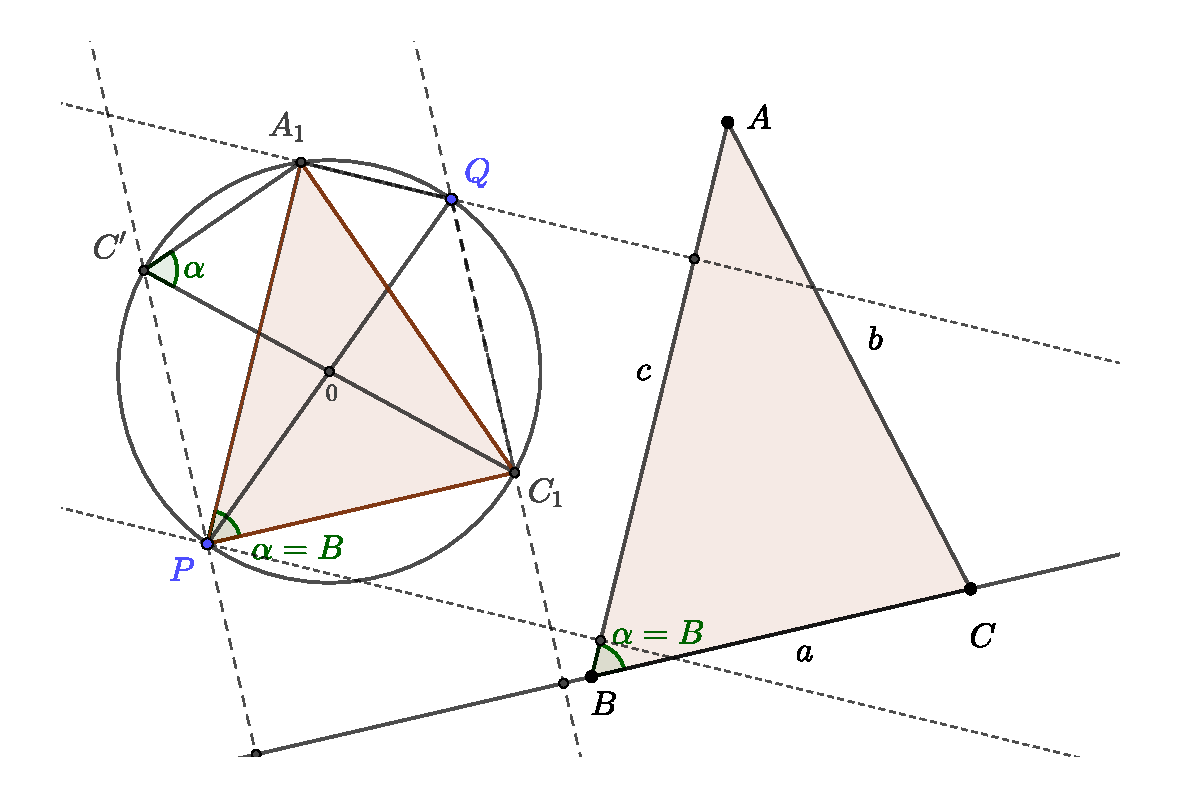
\includegraphics[scale=0.5]{pics_appA_060_distancia_trilinear.pdf}
			%
			\caption { \label{fig:distance_tri}   Distance between two points $P$ and $Q$.}
		\end{center}
	\end{figure}
By the law of cosines we have that
\[ |A_1-C_1|^2=|P-A_1|^2+|P-C_1|^2-2|P-A_1| \;|P-C_1| \cos \alpha \]

Since $C_1C'$ is a diameter it follows that $\angle A_1PC_1=\angle A_1C'C_1$. Therefore,
\[  |A_1-C_1|=|C-C'| \sin\alpha= |P-Q|\sin\alpha= \rho \sin B.\]
Now, by the construction of $A_1$ and $C_1$, we have that
\[ |P-C_1|= |p_1-p_2|,\;\;\;  |P-A_1|=| r_1-r_2|.\]
	This ends the proof.
\end{proof}

Let \[L=\left| \begin{matrix} q_1&r_1\\
q_2&r_2 \end{matrix} \right|, \;\;M=\left| \begin{matrix} r_1&p_1\\
r_2&p_2 \end{matrix} \right|,\;\; N=\left| \begin{matrix} p_1&q_1\\
p_2&q_2 \end{matrix} \right|   \]

Denote
\[ \{L,M,N\}= L^2+
M^2+N^2-2MN\cos A-2LN\cos B-2LM\cos C. 
\]

\begin{proposition}
	
	\[\rho^2=\frac{R^2 \{L,M,N\}}
	{\Delta^2}.\] 
	\end{proposition}
	
	
\begin{proof} The result follows from algebraic manipulations of the three formulas obtained in \cref{prop:distancePQ}. The details are left to the reader.
\end{proof}

\begin{proposition} Let $lx+my+nz=0$ be a straight line.
	Then the distances of the
	vertices of a reference triangle $ABC$ to this line are:
	
	\[p= \frac{2\Delta}{a}\frac{l}{\{l,m,n\}},\;\;
	%
	q=\frac{2\Delta}{b}\frac{m}{
		\{l,m,n\}},\;\;
 r=\frac{2\Delta}{c }\frac{n}{
 \{l,m,n\}}.\]
 
	
\end{proposition}



Two rays $CP$ and $CP'$ are called {\em  isogonal } relative to $C$ when $\angle ACP=\angle BCP'$. Equivalently, the ray $CX_1$ is a the common bisector of $P'CP$ and $ACB$.
If the analogous rays $AP$ and $AP'$ are isogonal ($\angle BAP=\angle BAP'$) we say that the points $P$ and $P'$ are {\em isogonal conjugates}. It can be shown that    
$\angle PBC=\angle P'BC$. 

\begin{proposition} Let  $P$ and $P'$ be isogonal conjugates. If $P=[p,q,r]$ then $P'=[1/p,1/q,1/r]=[qr,pr,pq]$. The map $\varphi(P)= P'$ is an involution, i.e., $\varphi^2=id$.
\end{proposition}

\begin{proof}
 
\end{proof}

\begin{proposition} Consider a triangle $T=ABC$. The points $X_3$ (circumcenter $O$) and $X_4$ (orthocenter $H$)  of $T$ are  isogonal conjugates.  
\end{proposition}

\begin{proof} 
	Consider the triangle $ABC$ and the circumcircle centered at $O=X_3$. The isosceles triangle $BOC$ has  angle $2A$ (or $2\pi-2A) $ at the vertex $O$. Therefore the angle between the ray $CO$ and the segment $BC$ is equal to $\pi/2-A$ (or $A-\pi/2$ ). The  angle between the ray $CX_4$ and the segment $CA$ is $\pi/2-A$ (or $A-\pi/2$ ). Therefore, $X_4=H$ and $X_3=O$ are isogonal relative to $C$. The same conclusion follows for the other vertices. 
		\begin{figure}[H]\ 
		\begin{center}
		 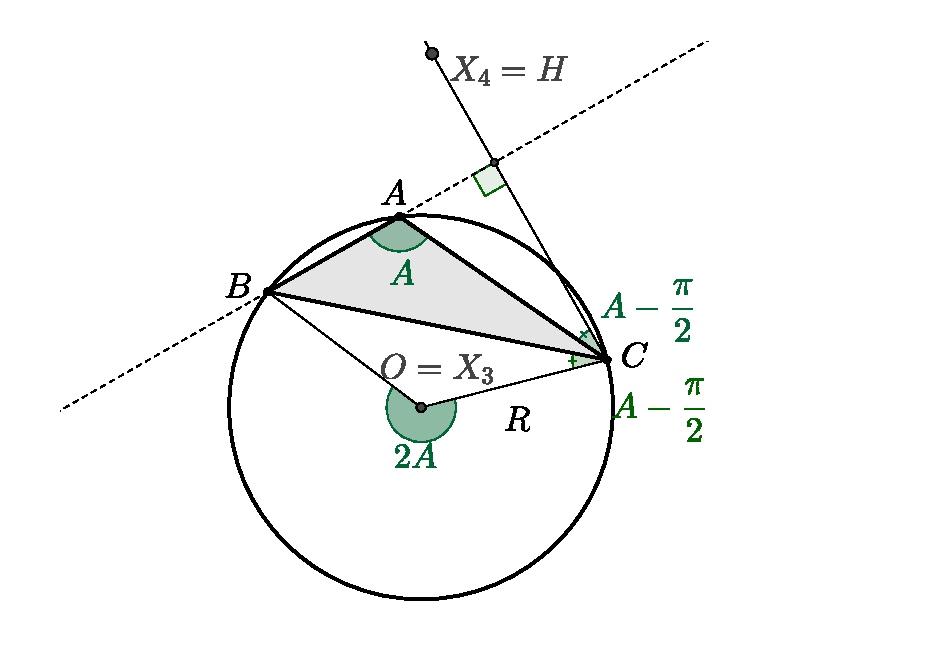
\includegraphics[width=.5\textwidth]{pics_appA_080_isogonalX3X4.pdf}
			\caption { \label{fig:X3X4}   Isogonal conjugate points $X_3$ and $X_4$.}
		\end{center}
	\end{figure}
\end{proof}


\section{Euler Line}

The Euler is a line passing through the pair of isogonal conjugate points $X_3$ and $X_4$.

The equation of Euler line in trilinear coordinates is given by

\begin{align*}
	 \left| \begin{matrix} x& y & z\\
	 	\cos A &\cos B &\cos C\\
	 	\frac{1}{\cos A}& \frac{1}{\cos B}& \frac{1}{\cos C} \end{matrix}
	 \right|=0,\; \\
%	 
\end{align*}
Developing the calculations it follows that the Euler line is given by:

\[  \cos A   (  \cos ^  {2}B - \cos^{2}C
) x+\cos B \left( \cos ^{2} C  -\cos^2 A 
\right) y+\cos C \left(   \cos  ^{2}A-  \cos ^2 B   \right) z=0.\]

In terms of the sides $a$, $b$ and $c$, the Euler line is given by:
\[a(c^2 - b^2) (-a^2 + b^2 + c^2)x + b(a^2 - c^2) (a^2 - b^2 + c^2)y + c(b^2 - a^2) (a^2 + b^2 - c^2)z=0
\]
The point at infinity in the Euler line is the intersection of the Euler line with the line  $ax+by+cz=0$ ( or equivalently 
$\sin A \;x+\sin B\; y+\sin C \; z=0$).

A notable point in the Euler line is the barycenter $X_2$,  which has trilinear coordinates
$[1/a,1/b,1/c]\equiv [\sin A, \sin B, \sin C]$. 



\begin{proposition}\label{prop:circumcircle_tri} Let $T=ABC$ be a triangle.
	The circumcircle in trilinear coordinates is given by
	\[a y z+b x z+c x y=0.\]
\end{proposition}

\begin{proof}
	
	\end{proof}
	
	\begin{proposition}
	    Consider the triangle $A=[\alpha,\beta]$, $B=[-1,0], C=[1,0]$.
	    The Euler line is given by:
	   \[ (3-3\alpha^2 - \beta^2  )x - 2\alpha \beta y + \alpha(\alpha^2 + \beta^2 - 1)=0\]
	\end{proposition}
	
	\begin{proof} In cartesian coordinates:
	\[ X_3=[0, \frac{\alpha^2 + \beta^2 - 1}{2\beta}],\;\; X_4=[\alpha, \frac{1-\alpha^2  }{\beta}]
	\]
	 Therefore the result follows from direct calculations.   
	\end{proof}
	